\documentclass[11pt]{scrreprt}
\usepackage[T1]{fontenc}
\usepackage[utf8]{inputenc}
\usepackage[french]{babel}
\usepackage[scale=0.775]{geometry}
\usepackage{lmodern}
\usepackage[ilines]{scrpage2}
\usepackage[pdftex, bookmarks=true, hidelinks]{hyperref}
\usepackage{graphicx}
\usepackage{tocbibind}
\usepackage{chngcntr}
\usepackage{tabularx}
\usepackage{float}
\usepackage{scrhack}
\usepackage{ulem}

\counterwithout{figure}{chapter}
\counterwithout{table}{chapter}
\pagestyle{scrheadings}

% clear head and foot
\clearscrheadings
\clearscrplain
\clearscrheadfoot

\cefoot[\textsc{Nathan Raspe \& Matteo Taroli}]{\textsc{Nathan Raspe \& Matteo Taroli}}
\cofoot[\textsc{Nathan Raspe \& Matteo Taroli}]{\textsc{Nathan Raspe \& Matteo Taroli}}
\lefoot[]{}
\lofoot[]{}
\refoot[\thepage]{\thepage}
\rofoot[\thepage]{\thepage}

\begin{document}

    \renewcommand{\labelitemi}{$\bullet$}
    \renewcommand{\labelitemii}{$\circ$}
    %%%%%% TITLE PAGE %%%%%%%%%%%%%%%%%%%
    \begin{titlepage}
        \begin{center}
            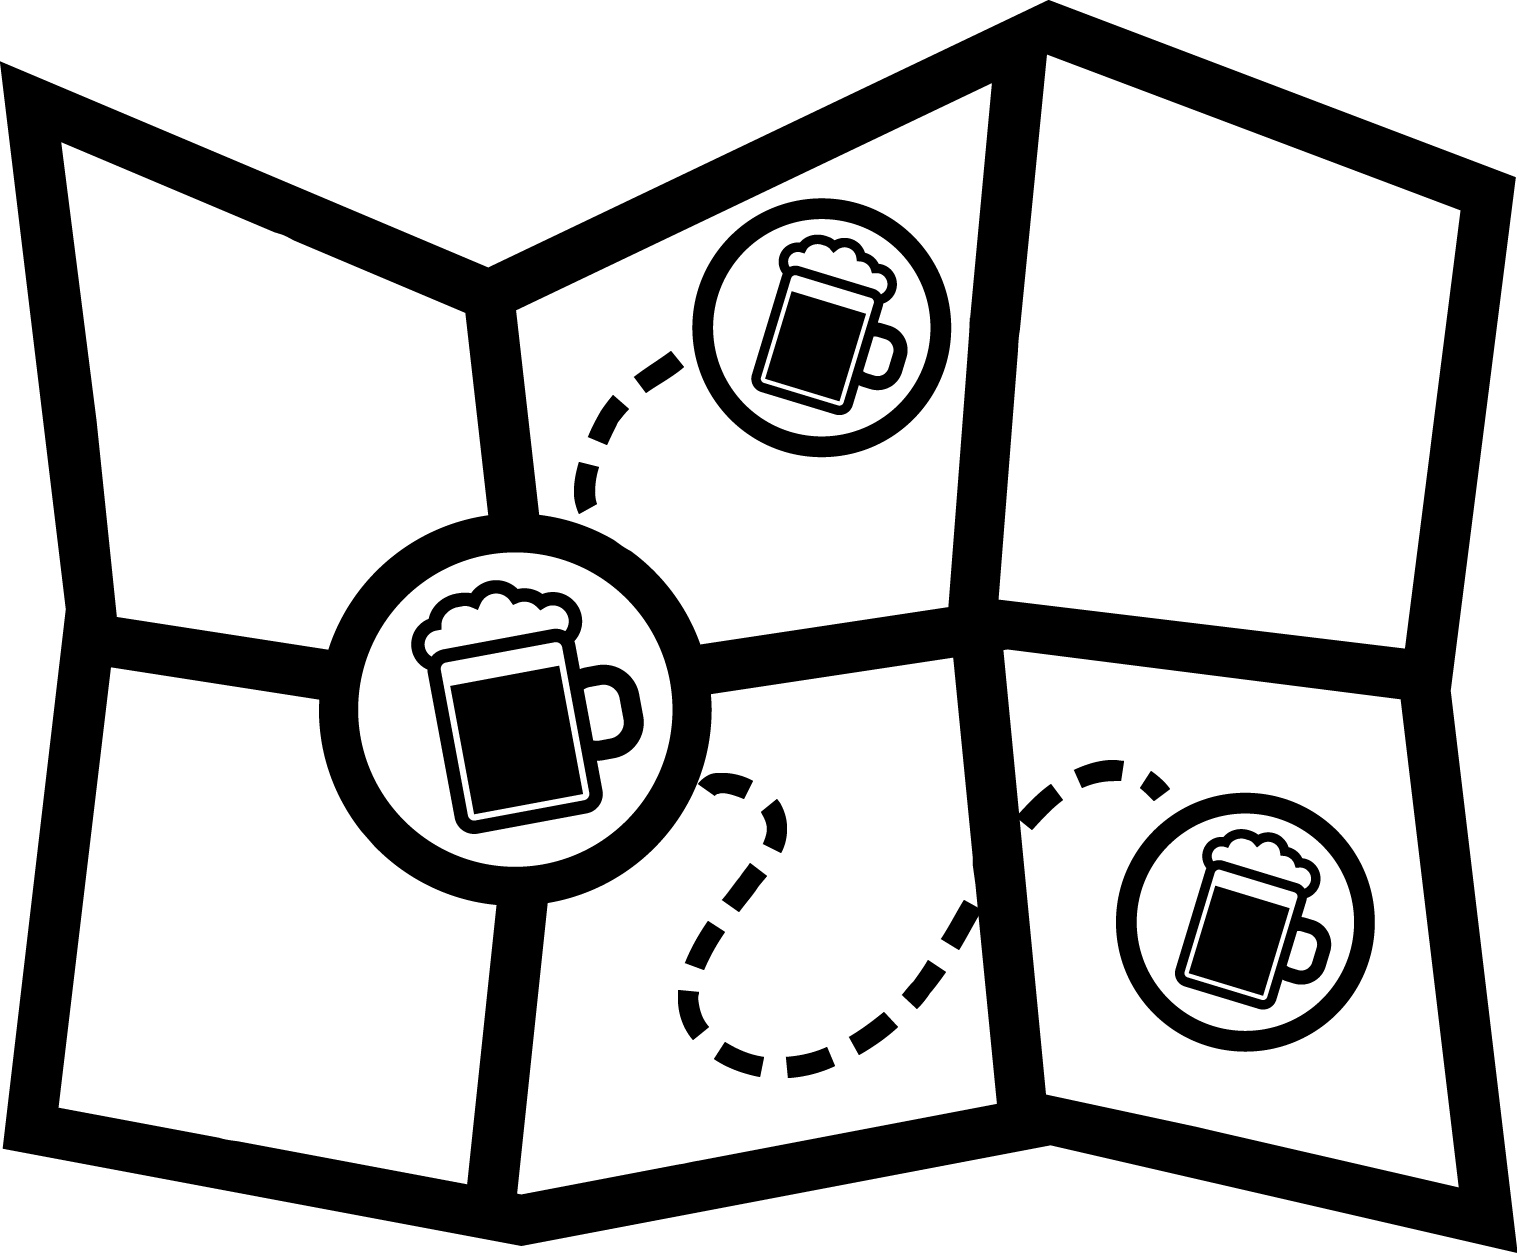
\includegraphics[width=10cm]{images/logo.png}
            ~\\[1.5cm]

            % Title
            \rule{\textwidth}{1pt} \\[0.4cm]
            \Huge{\textsc{\textbf{History Pub}}}\\ \Large{\textit{Découvrez Soignies en boisson}\\[0.4cm]}

            \rule{\textwidth}{1pt} \\[1.5cm]

            \textsc{\Large Projet de Développement d'Application Mobile}\\[0.5cm]

            % Authors
            Nathan Raspe \& Matteo Taroli

            \vfill

            {\large 27 Novembre 2015}
            \vfill
        \end{center}
    \end{titlepage}

    % Table of contents
    \pagenumbering{roman}
    \tableofcontents
    % List of figures
    \renewcommand\listfigurename{Table des illustrations}
    \listoffigures
    \pagebreak
    \pagenumbering{arabic}

    %%%%%%%% BEGIN CONTENT %%%%%%%%%%%%
    \chapter{Introduction}
    Dans le cadre du cours de Dévelopement d'Application Mobile, nous avons du développer une application reprenant le concept du jeu de piste. Cette application, nommée \textsc{History Pub} vous propose de découvrir la ville de Soignies en passant par les différents bars que la ville offre.

    Sur le chemin entre ces différents établissements, vous aurez l'occasion d'en apprendre plus sur l'histoire et le folklore de la ville. Durant les différents arrêts, vous aurez bien entendu l'occasion de profiter des bar et des diverses boissons proposées avant de reprendre le chemin vers d'autres découvertes!

    Attention tout de même, l'alcool est à consommer avec modération, sous peine de ne plus pouvoir répondre aux questions données!

    \chapter{Mode d'emploi}
    L'utilisation de \textsc{History Pub} est très facile. Une fois l'application lancée, le jeu ne démarre réellement qu'une fois que vous vous trouvez dans la zone de jeu, qui vous est logiquement donnée.

    % Afficher une screenshot de EtapeActivité demandant de se déplacer dans la zone

    Une fois dans la zone, et après avoir lu une courte description de l'endroit et où de son histoire, vous vous retrouverez devant une épreuve qui peut prendre différentes formes. Ces épreuves sont décrites ci-dessous.

    \section{Epreuve Question à Choix Multiple}
    % mettre un screenshot et expliquer vite fait
    %   - comment on choisit une réponse
    %   - comment on gère si pas de réponse
    %   - comment on affiche si c'est bon ou pas

    \section{Epreuve Question Ouverte}
    % mettre un screenshot et expliquer vite fait
    %   - comment on choisit une réponse
    %   - comment on gère si pas de réponse
    %   - comment on affiche si c'est bon ou pas


    \section{Epreuve Photographie}
    % mettre un screenshot et expliquer vite fait
    %   - comment on choisit une réponse
    %   - comment on gère si pas de réponse
    %   - comment on affiche si c'est bon ou pas


    \chapter{Architecture}

    \chapter{Bugs connus}
    % Aucun bug connu pour le moment :P

    \chapter{Utilisation de code open-source}
    Le code de \textsc{History Pub} n'utilise pas réellement de code open-source à proprement parler. Cependant, certaines parties sont fortement inspirées, voire même simplement reprises, des exemples et tutoriels fournis par \textsc{Google} sur leur plateforme \url{developer.android.com}.

    La partie géolocalisation par exemple est principalement une copie de leur exemple, adapté à nos besoins.

    \chapter{License}

    \noindent \textsc{History Pub} est placé sous license GNU GENERAL PUBLIC LICENSE version 3.
    \hfill\\

    \noindent Cela signifie que n'importe qui \textbf{peut} :
    \begin{itemize}
        \item utiliser notre code de façon privée
        \item utiliser notre code dans des projets à but commercial
        \item redistribuer notre code
        \item modifier notre code
    \end{itemize}
    \hfill\\
    Mais cela signifie aussi qu'une personne utilisant tout ou partie du code de \textsc{History Pub} dans un projet \textbf{doit} :
    \begin{itemize}
        \item publier les sources de ce projet
        \item inclure une copy de la license et copyright dans ce projet
        \item préciser les changements importants fait à notre code
    \end{itemize}
    \hfill\\
    Celà signifie aussi que notre code est fourni sans garantie et que nous ne pouvons donc pas être tenus responsable de problèmes quelconques liés à son utilisation en dehors de \textsc{History Pub}.
    \hfill\\

    \noindent Pour plus d'information, la license complète peut être trouvée à l'adresse suivante : \url{https://www.gnu.org/licenses/gpl.html}

\end{document}
